The ifo Business Survey is a monthly poll conducted since 1949 by the ifo Institute
for Economic Research in Germany, gathering responses from multiple firms
across different sectors \citep{sauer2023handbook}. It includes self-assessment questions on topics such as the current business situation or expectation and also more specific questions, such as production plans. The answers are aggregated hierarchically, ranging from small specific industries up to four main sectors: manufacturing industry, construction industry, service sector and trade. The survey's most popular indicator is the ifo Business Climate Index, consisting of the the two questions on current business situation and expectation, aggregated across all industries. The index is well-established as a leading indicator, with many studies examining its predictive power for economic variables such as the national GDP. However, the underlying structures within the business survey are largely unexplored so far. In this project, we will take a closer look on the many time series underlying the ifo Business Climate Index. Rather than focusing on building a rigorously validated predictive model, this project seeks to uncover potential relationships in these time series through a descriptive analysis of historical data.


\begin{figure}[H]
    \centering
    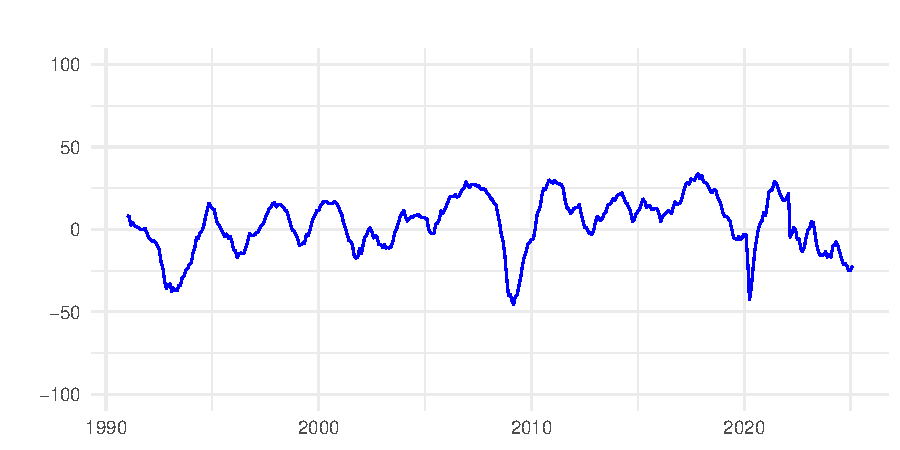
\includegraphics[width=0.5\linewidth]{JakobPlots/main_index_plot.pdf}
    \caption{ifo Business Climate Index over the period considered in this analysis.}
    \label{fig:main_index}
\end{figure}

\subsubsection{Data}
Within the survey, we focus on the manufacturing sector, one of the main drivers of the German economy \citep{sauer2023handbook}. In our dataset, the highest aggregation level corresponds to the entire manufacturing sector as a whole. One level below this aggregate in the hierarchical structure, there are 21 constituent industries such as the automotive industry or the machinery and equipment industry. We refer to these as level~1 aggregates. In total, five levels exist, though our analysis mainly considers level~1 and level~2 aggregates. Industry aggregates are identified by an industry code based on the official classification of economic activities of the German Federal Statistical Office \citep{sauer2023handbook}. For example, the main aggregate is coded \texttt{C0000000}, with the letter \texttt{C} denoting the manufacturing industry and the digits indicating the aggregation level, which is the the highest level in this case, as all digits are zero. Industries at level~1 are identified by the first two digits, e.g.\ \texttt{C2800000} for machinery and equipment. Each additional nonzero digit specifies one further level, so \texttt{C2810000} corresponds to a level~2 sub-aggregate of machinery. In our study we define level~1 aggregates (codes \texttt{C} followed by two digits) as sectors. Table~\ref{tab:sectors} provides an overview of the manufacturing sectors covered by the survey. The abbreviations for all other industry codes can be found in the appendix~\ref{ch:appendix}.

\begin{table}[H]
    \centering
    \small
    \begin{tabularx}{\textwidth}{lX}
        \toprule
        \textbf{Code} & \textbf{Sector} \\
        \midrule
        C1000000 & Manufacture of food products \\
        C1100000 & Manufacture of beverages \\
        C1300000 & Manufacture of textiles \\
        C1400000 & Manufacture of wearing apparel \\
        C1500000 & Manufacture of leather and related products \\
        C1600000 & Manufacture of wood and of products of wood and cork, except furniture; manufacture of articles of straw and plaiting materials \\
        C1700000 & Manufacture of paper and paper products \\
        C1800000 & Printing and reproduction of recorded media \\
        C1900000 & Manufacture of coke and refined petroleum products \\
        C2000000 & Manufacture of chemicals and chemical products \\
        C2100000 & Manufacture of basic pharmaceutical products and pharmaceutical preparations \\
        C2200000 & Manufacture of rubber and plastic products \\
        C2300000 & Manufacture of other non-metallic mineral products \\
        C2400000 & Manufacture of basic metals \\
        C2500000 & Manufacture of fabricated metal products, except machinery and equipment \\
        C2600000 & Manufacture of computer, electronic and optical products \\
        C2700000 & Manufacture of electrical equipment \\
        C2800000 & Manufacture of machinery and equipment n.e.c. \\
        C2900000 & Manufacture of motor vehicles, trailers and semi-trailers \\
        C3000000 & Manufacture of other transport equipment \\
        \bottomrule
    \end{tabularx}
    \caption{Overview of manufacturing sectors covered by the ifo Business Survey}
    \label{tab:sectors}
\end{table}

The ifo survey covers multiple questions on the current situation and expectations. For consistency, we restrict our analysis to questions and aggregates that have been included continuously from 1991 up to February 2025, the last month in our dataset. Furthermore, we only include questions that are asked on a monthly basis to avoid mixing indices of different frequencies (monthly, quarterly, or yearly). Aggregates with any missing values for a given question during this period were excluded. Table~\ref{tab:ifo_terms} lists the survey questions and their corresponding abbreviations.

\begin{table}[H]
\small
\centering
\label{tab:ifo_terms}
\begin{tabularx}{\textwidth}{|r|l|X|}
\toprule
\textbf{Abbreviation} & \textbf{German Term} & \textbf{English Translation} \\
\midrule
KLD & Geschäftsklima & Business Climate \\
GUS & Geschäftslage Beurteilung & Business Situation Assessment \\
GES & Geschäftslage Erwartungen & Business Situation Expectations \\
LUS & Fertigwarenlager Beurteilung & Finished Goods Inventory Assessment \\
BUS & Auftragsbestand Beurteilung & Order Backlog Assessment \\
XUS & Auftragsbestand Beurteilung Export & Export Order Backlog Assessment \\
AVS & Nachfrage gegen Vormonat & Demand compared to Previous Month \\
BVS & Auftragsbestand gegen Vormonat & Order Backlog compared to Previous Month \\
QVS & Produktion gegen Vormonat & Production compared to Previous Month \\
PVS & Preise gegen Vormonat & Prices compared to Previous Month \\
QES & Produktionspläne & Production Plans \\
PWS & Preiserwartungen & Price Expectations \\
XES & Exporterwartungen & Export Expectations \\
BES & Beschäftigtenerwartungen & Employment Expectations \\
PRS & Produktivitätserwartungen & Productivity Expectations \\
\bottomrule
\end{tabularx}
\caption{ifo Business Survey questions and their translations.}
\label{tab:ifo_terms}
\end{table}

In our analysis we define the level~0 aggregate of the business climate question (KLD) for the manufacturing sector as the main index, which serves as the central reference point throughout the study.

